Created by tikzDevice version 0.5.3 on 2011-03-04 16:41:47
% \documentclass{article}
% \usepackage{tikz}

% \usepackage[active,tightpage]{preview}

% \PreviewEnvironment{pgfpicture}

% \setlength\PreviewBorder{0pt}
% \begin{document}
%-----------------------------------
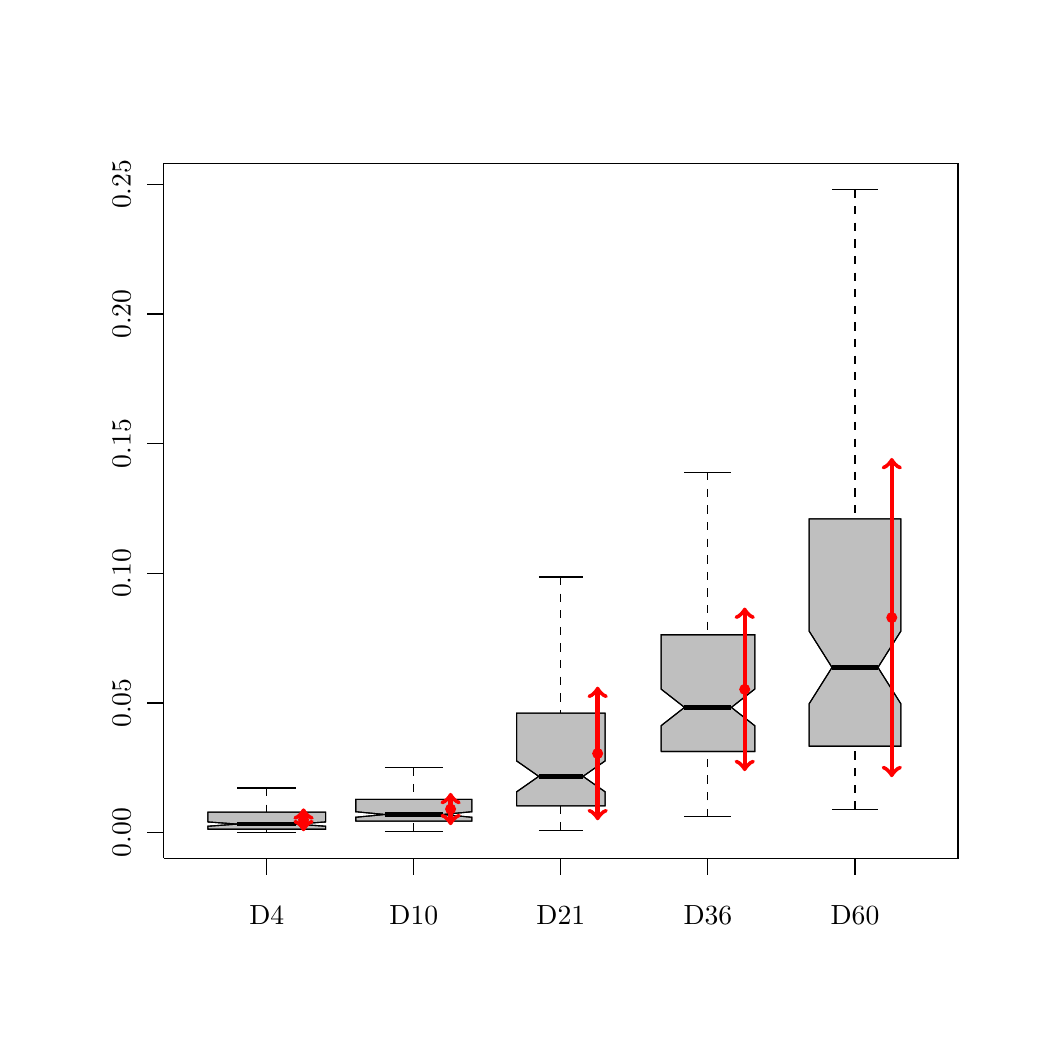
\begin{tikzpicture}[x=1pt,y=1pt]
\begin{scope}
\draw[fill=lightgray] ( 65.14, 71.70) --
	(107.65, 71.70) --
	(107.65, 72.79) --
	( 97.02, 73.56) --
	(107.65, 74.34) --
	(107.65, 77.88) --
	( 65.14, 77.88) --
	( 65.14, 74.34) --
	( 75.77, 73.56) --
	( 65.14, 72.79) --
	cycle;

\draw[ultra thick] ( 75.77, 73.56) -- ( 97.02, 73.56);

\draw[dashed] ( 86.40, 70.49) -- ( 86.40, 71.70);

\draw[dashed] ( 86.40, 86.59) -- ( 86.40, 77.88);

\draw[] ( 75.77, 70.49) -- ( 97.02, 70.49);

\draw[] ( 75.77, 86.59) -- ( 97.02, 86.59);

\draw[] ( 65.14, 71.70) --
	(107.65, 71.70) --
	(107.65, 72.79) --
	( 97.02, 73.56) --
	(107.65, 74.34) --
	(107.65, 77.88) --
	( 65.14, 77.88) --
	( 65.14, 74.34) --
	( 75.77, 73.56) --
	( 65.14, 72.79) --
	( 65.14, 71.70);

\draw[fill=lightgray] (118.55, 74.63) --
	(160.52, 74.63) --
	(160.52, 76.03) --
	(150.03, 77.03) --
	(160.52, 78.03) --
	(160.52, 82.51) --
	(118.55, 82.51) --
	(118.55, 78.03) --
	(129.04, 77.03) --
	(118.55, 76.03) --
	cycle;

\draw[ultra thick] (129.04, 77.03) -- (150.03, 77.03);

\draw[dashed] (139.54, 70.95) -- (139.54, 74.63);

\draw[dashed] (139.54, 94.09) -- (139.54, 82.51);

\draw[] (129.04, 70.95) -- (150.03, 70.95);

\draw[] (129.04, 94.09) -- (150.03, 94.09);

\draw[] (118.55, 74.63) --
	(160.52, 74.63) --
	(160.52, 76.03) --
	(150.03, 77.03) --
	(160.52, 78.03) --
	(160.52, 82.51) --
	(118.55, 82.51) --
	(118.55, 78.03) --
	(129.04, 77.03) --
	(118.55, 76.03) --
	(118.55, 74.63);

\draw[fill=lightgray] (176.68, 80.12) --
	(208.67, 80.12) --
	(208.67, 85.22) --
	(200.67, 90.81) --
	(208.67, 96.39) --
	(208.67,113.67) --
	(176.68,113.67) --
	(176.68, 96.39) --
	(184.68, 90.81) --
	(176.68, 85.22) --
	cycle;

\draw[ultra thick] (184.68, 90.81) -- (200.67, 90.81);

\draw[dashed] (192.67, 71.28) -- (192.67, 80.12);

\draw[dashed] (192.67,162.86) -- (192.67,113.67);

\draw[] (184.68, 71.28) -- (200.67, 71.28);

\draw[] (184.68,162.86) -- (200.67,162.86);

\draw[] (176.68, 80.12) --
	(208.67, 80.12) --
	(208.67, 85.22) --
	(200.67, 90.81) --
	(208.67, 96.39) --
	(208.67,113.67) --
	(176.68,113.67) --
	(176.68, 96.39) --
	(184.68, 90.81) --
	(176.68, 85.22) --
	(176.68, 80.12);

\draw[fill=lightgray] (228.87, 99.80) --
	(262.75, 99.80) --
	(262.75,109.10) --
	(254.28,115.73) --
	(262.75,122.36) --
	(262.75,141.97) --
	(228.87,141.97) --
	(228.87,122.36) --
	(237.34,115.73) --
	(228.87,109.10) --
	cycle;

\draw[ultra thick] (237.34,115.73) -- (254.28,115.73);

\draw[dashed] (245.81, 76.17) -- (245.81, 99.80);

\draw[dashed] (245.81,200.72) -- (245.81,141.97);

\draw[] (237.34, 76.17) -- (254.28, 76.17);

\draw[] (237.34,200.72) -- (254.28,200.72);

\draw[] (228.87, 99.80) --
	(262.75, 99.80) --
	(262.75,109.10) --
	(254.28,115.73) --
	(262.75,122.36) --
	(262.75,141.97) --
	(228.87,141.97) --
	(228.87,122.36) --
	(237.34,115.73) --
	(228.87,109.10) --
	(228.87, 99.80);

\draw[fill=lightgray] (282.35,101.68) --
	(315.55,101.68) --
	(315.55,116.98) --
	(307.25,130.16) --
	(315.55,143.34) --
	(315.55,183.85) --
	(282.35,183.85) --
	(282.35,143.34) --
	(290.65,130.16) --
	(282.35,116.98) --
	cycle;

\draw[ultra thick] (290.65,130.16) -- (307.25,130.16);

\draw[dashed] (298.95, 78.85) -- (298.95,101.68);

\draw[dashed] (298.95,302.86) -- (298.95,183.85);

\draw[] (290.65, 78.85) -- (307.25, 78.85);

\draw[] (290.65,302.86) -- (307.25,302.86);

\draw[] (282.35,101.68) --
	(315.55,101.68) --
	(315.55,116.98) --
	(307.25,130.16) --
	(315.55,143.34) --
	(315.55,183.85) --
	(282.35,183.85) --
	(282.35,143.34) --
	(290.65,130.16) --
	(282.35,116.98) --
	(282.35,101.68);
\end{scope}
\begin{scope}
\path[clip] (  0.00,  0.00) rectangle (361.35,361.35);
\definecolor[named]{drawColor}{rgb}{0.00,0.00,0.00}

\draw[] ( 86.40, 61.20) -- (298.95, 61.20);

\draw[] ( 86.40, 61.20) -- ( 86.40, 55.20);

\draw[] (139.54, 61.20) -- (139.54, 55.20);

\draw[] (192.67, 61.20) -- (192.67, 55.20);

\draw[] (245.81, 61.20) -- (245.81, 55.20);

\draw[] (298.95, 61.20) -- (298.95, 55.20);

\node[anchor=base,inner sep=0pt, outer sep=0pt] at ( 86.40, 37.20) {D4%
};

\node[anchor=base,inner sep=0pt, outer sep=0pt] at (139.54, 37.20) {D10%
};

\node[anchor=base,inner sep=0pt, outer sep=0pt] at (192.67, 37.20) {D21%
};

\node[anchor=base,inner sep=0pt, outer sep=0pt] at (245.81, 37.20) {D36%
};

\node[anchor=base,inner sep=0pt, outer sep=0pt] at (298.95, 37.20) {D60%
};

\draw[] ( 49.20, 70.47) -- ( 49.20,304.73);

\draw[] ( 49.20, 70.47) -- ( 43.20, 70.47);

\draw[] ( 49.20,117.32) -- ( 43.20,117.32);

\draw[] ( 49.20,164.18) -- ( 43.20,164.18);

\draw[] ( 49.20,211.03) -- ( 43.20,211.03);

\draw[] ( 49.20,257.88) -- ( 43.20,257.88);

\draw[] ( 49.20,304.73) -- ( 43.20,304.73);

\node[rotate= 90.00,anchor=base,inner sep=0pt, outer sep=0pt] at ( 37.20, 70.47) {0.00%
};

\node[rotate= 90.00,anchor=base,inner sep=0pt, outer sep=0pt] at ( 37.20,117.32) {0.05%
};

\node[rotate= 90.00,anchor=base,inner sep=0pt, outer sep=0pt] at ( 37.20,164.18) {0.10%
};

\node[rotate= 90.00,anchor=base,inner sep=0pt, outer sep=0pt] at ( 37.20,211.03) {0.15%
};

\node[rotate= 90.00,anchor=base,inner sep=0pt, outer sep=0pt] at ( 37.20,257.88) {0.20%
};

\node[rotate= 90.00,anchor=base,inner sep=0pt, outer sep=0pt] at ( 37.20,304.73) {0.25%
};
\end{scope}
\begin{scope}
\path[clip] (  0.00,  0.00) rectangle (361.35,361.35);
\draw ( 49.20, 61.20) --
	(336.15, 61.20) --
	(336.15,312.15) --
	( 49.20,312.15) --
	( 49.20, 61.20);
\end{scope}
\begin{scope}
\path[clip] ( 49.20, 61.20) rectangle (336.15,312.15);

\fill[color=red] ( 99.68, 75.11) circle (2);
\fill[color=red] (152.82, 79.00) circle (2);
\fill[color=red] (205.96, 99.07) circle (2);
\fill[color=red] (259.10,122.25) circle (2);
\fill[color=red] (312.24,148.19) circle (2);

\draw[<->,ultra thick,color=red] ( 99.68, 70.97) -- ( 99.68, 79.25);
\draw[<->,ultra thick,color=red] (152.82, 73.17) -- (152.82, 84.83);
\draw[<->,ultra thick,color=red] (205.96, 74.94) -- (205.96,123.21);
\draw[<->,ultra thick,color=red] (259.10, 92.70) -- (259.10,151.80);
\draw[<->,ultra thick,color=red] (312.24, 90.51) -- (312.24,205.86);

\end{scope}
\end{tikzpicture}
%-----------------------------------
%\end{document}